\chapter{Results and discussion}

\section{RGCN is able to accurately predict expected water solubility}


% \begin{figure}[h]
%     \centering
%     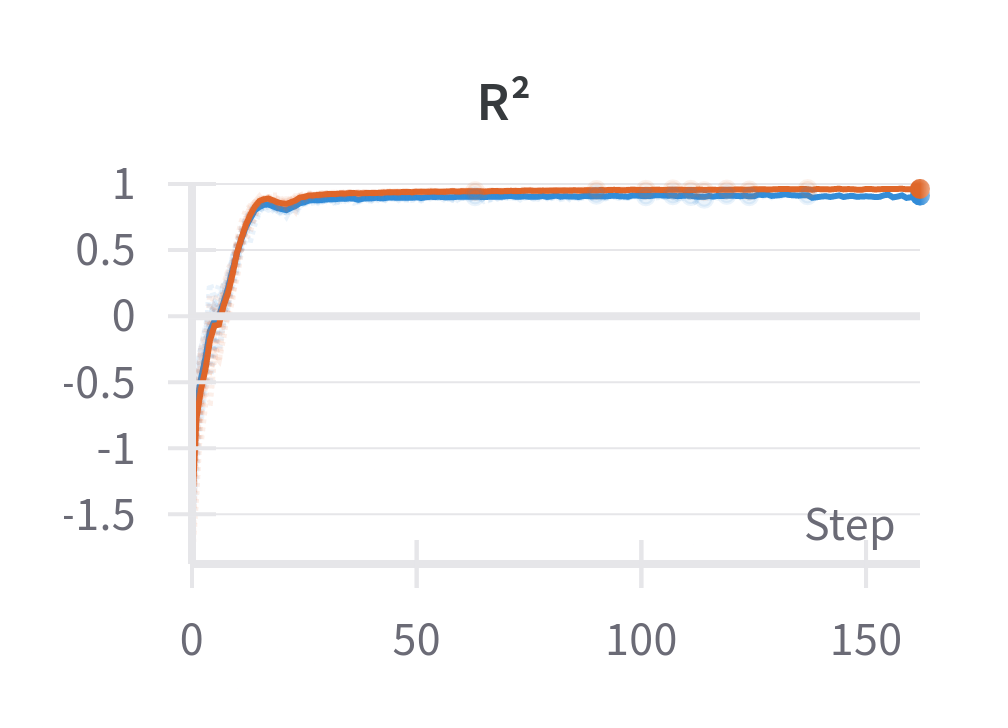
\includegraphics[scale=0.20]{rgcn_r2.png}
%     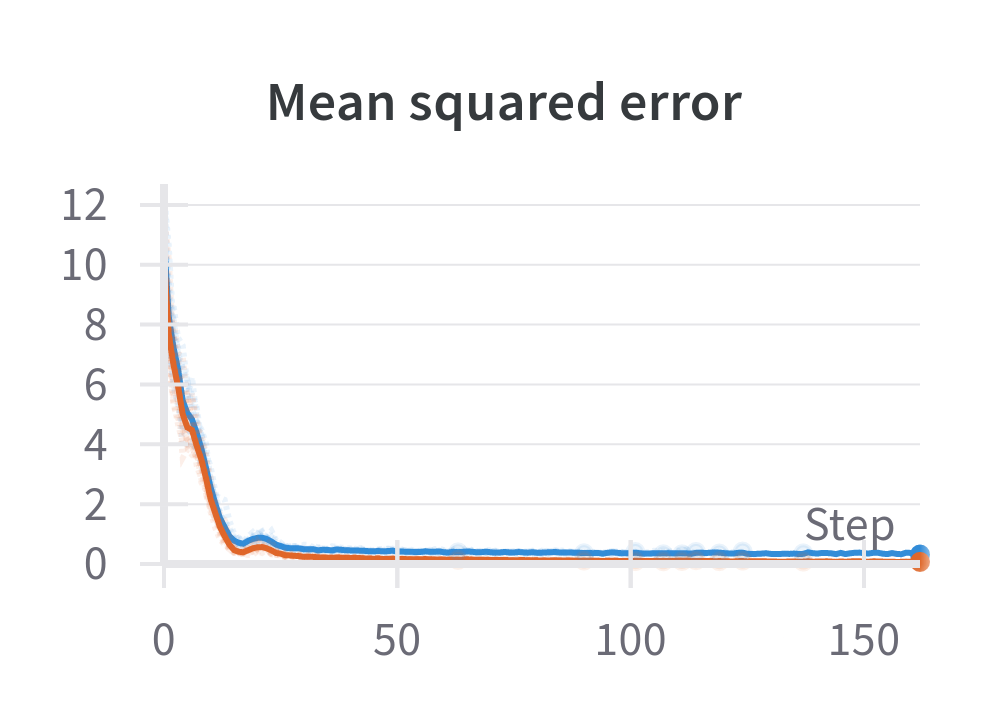
\includegraphics[scale=0.20]{rgcn_mse.png}
%     \caption{Average Mean squared error (left) and $R^2$ (right) of train (orange) and validation 
%     (blue) data during model training over the ten RGCN models, each trained using a different 
%     seed. Both metrics show a good model performance and no overfitting.}
% \end{figure}


\begin{figure}[h]
    \centering
    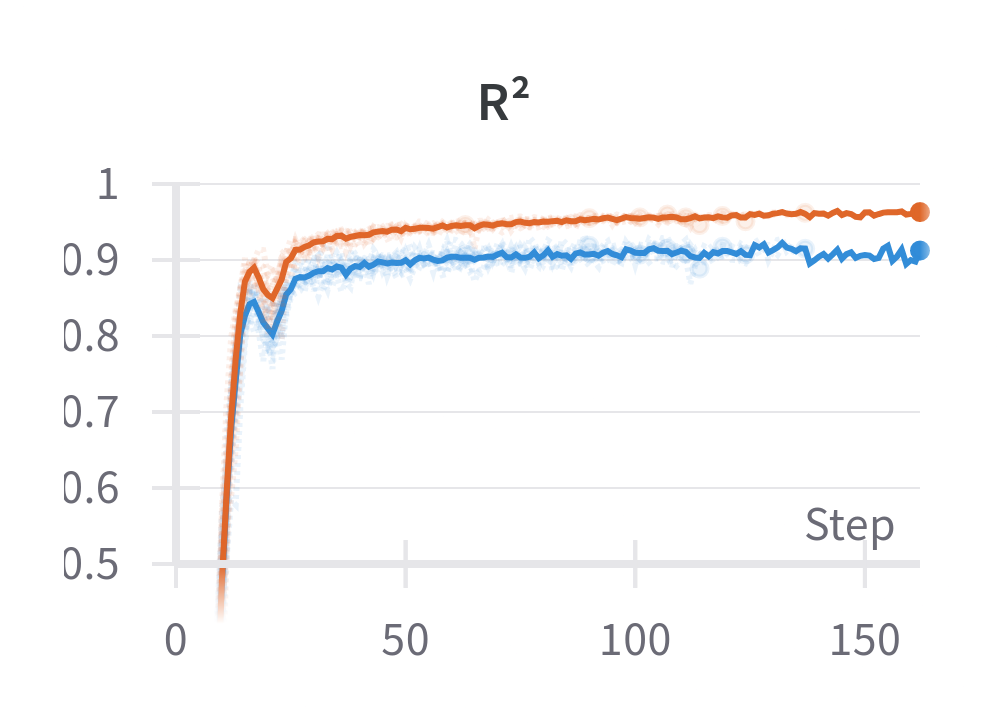
\includegraphics[scale=0.20]{rgcn_r2_zoomed.png}
    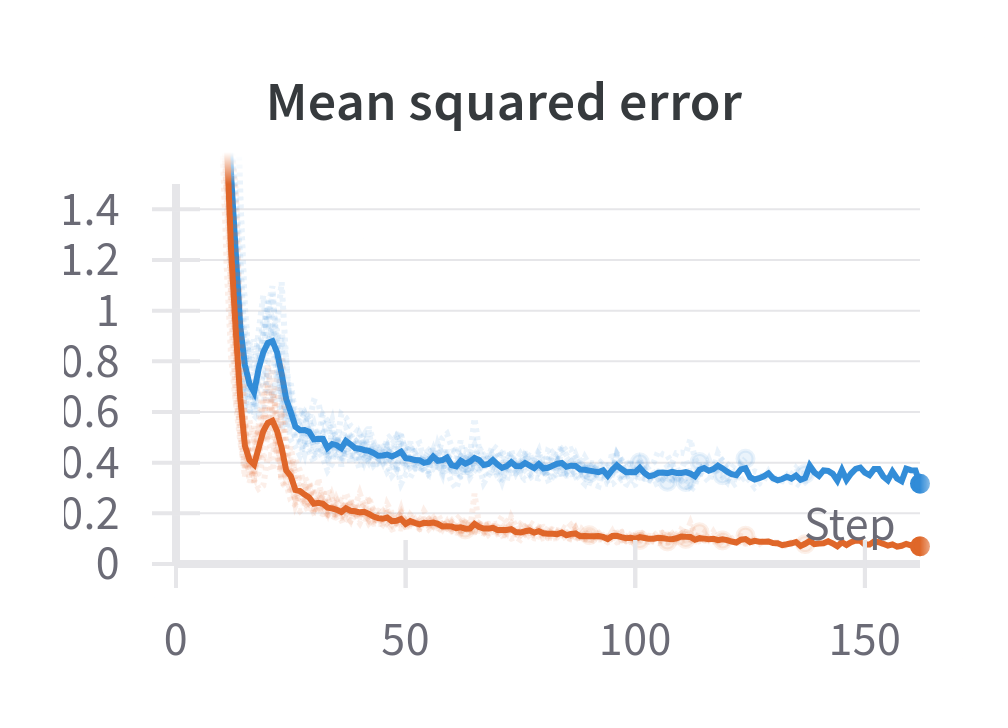
\includegraphics[scale=0.20]{rgcn_mse_zoomed.png}
    \caption{Average $R^2$ (left) and mean squared error (right) of train (orange) and validation 
    (blue) data during model training over the ten RGCN models, each trained using a different 
    seed. Both metrics show a good model performance and no overfitting. }
\end{figure}

\section{The absolute prediction error is not associated with the Spearman rank correlation between different attribution methods}


\begin{figure}[h]
    \centering
    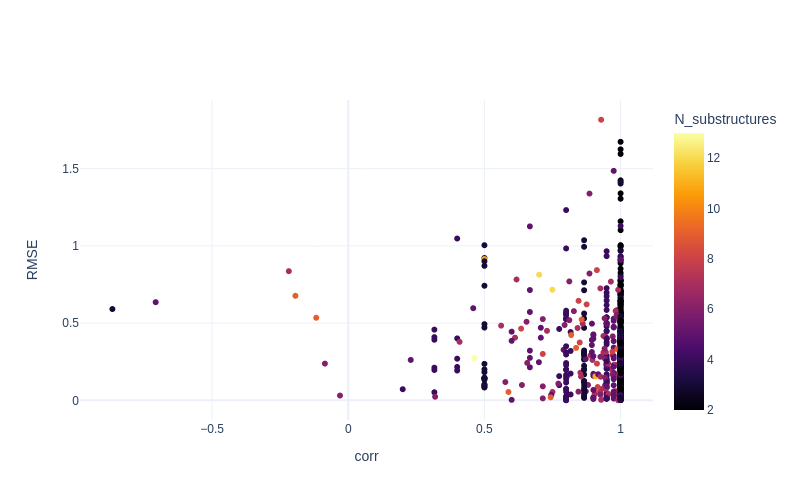
\includegraphics[scale=0.35]{../data/images/esol_rank_vs_AE_SME_Shapley_combined.png}
    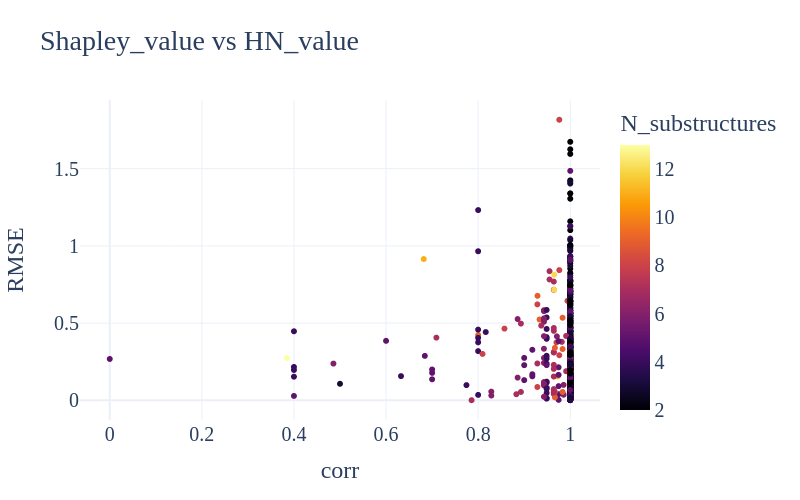
\includegraphics[scale=0.35]{../data/images/esol_rank_vs_AE_Shapley_HN_combined.png}
    \caption{Absolute error of model prediction in function of Spearman rank correlation between 
        attributions from SME and Shapley (top) and between Shapley and HN (bottom) using the full 
        data set containing 1110 molecules.
    }
\end{figure}


\section{Relative evaluation of attribution methods using chemically intuitively ranked substructures shows no statistical
significant difference between the attribution methods}

\begin{figure}[h]
    \centering
    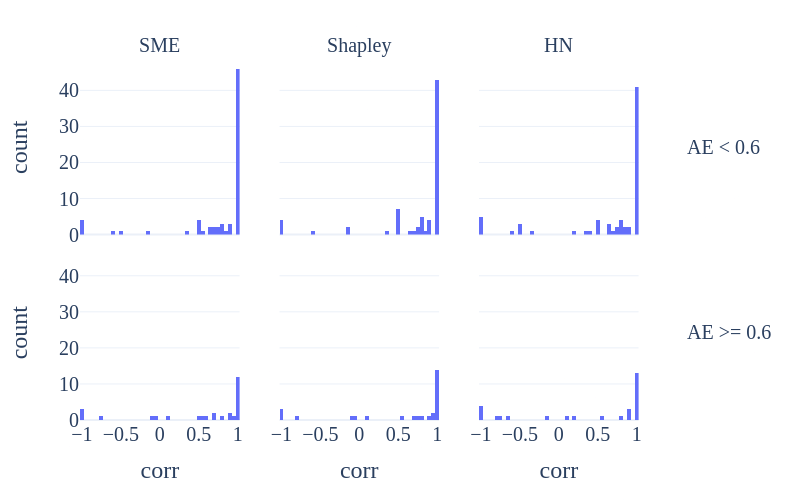
\includegraphics[scale=0.5]{spearman_rank_correlation_manual_vs_attribution.png}
    \caption{Distribution of Spearman rank correlation between an attribution method 
        and a manual ranking of substructures using chemical reasoning. The difference 
        between the two absolute error groups is mainly the intensity of high 
        correlation values.
    }
    \label{fig:spearman_corr_manual}
\end{figure}


\section{All attribution methods are equally faithful to the ML model}

\begin{figure}[h]
    \centering
    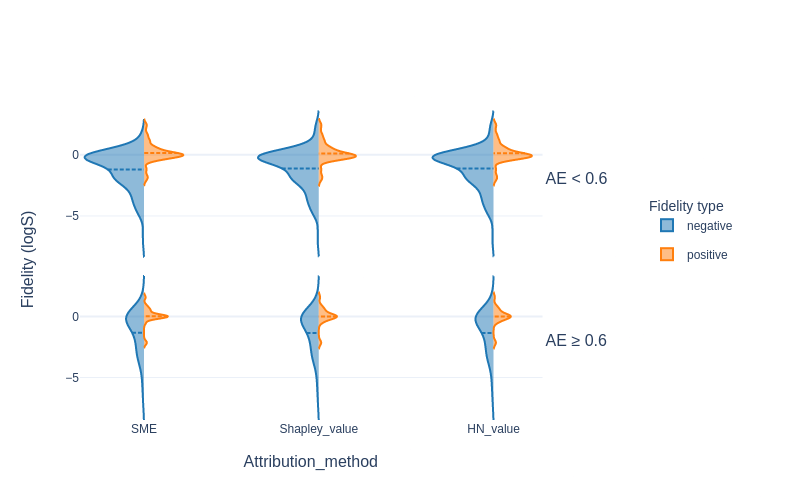
\includegraphics[scale=0.5]{fidelity.png}
    \caption{Distribution of fidelity obtained by removing the most positive 
        attribution (right side) or the most negative attribution (left side).
    }
    \label{fig:fidelity}
\end{figure}


\begin{figure}[h]
    \centering
    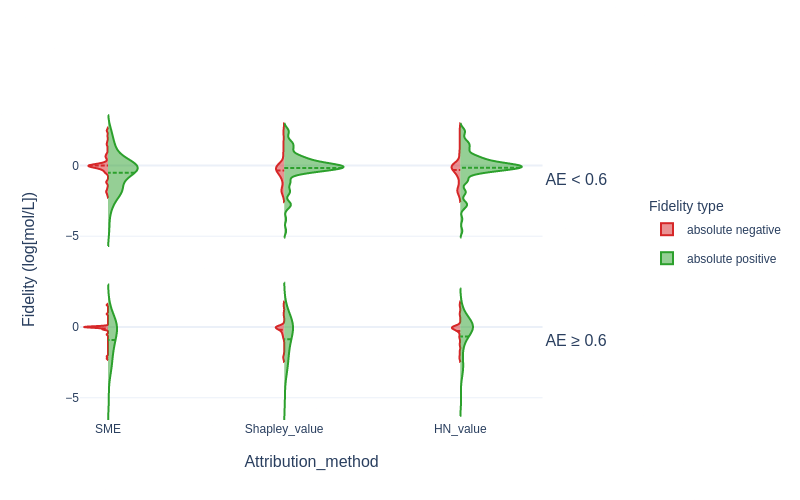
\includegraphics[scale=0.5]{absolute_fidelity.png}
    \caption{Distribution of fidelity obtained by removing the most positive 
        attribution in absolute values (right side) or the most negative 
        attribution in absolute values (left side).
    }
    \label{fig:fidelity}
\end{figure}
